\documentclass[a4paper]{article}

\usepackage[T2A]{fontenc}
\usepackage[russian]{babel}
\usepackage{graphicx}
\usepackage{float}
\usepackage{hyperref}
\usepackage{amsmath, amssymb}
\usepackage{caption}

\newcommand{\minus}{\scalebox{0.75}[1.0]{$-$}}


\title{\Huge{Физика}\\ Решение Овчинкина}
\author{\huge{Евгений Турчанин}}
\date{}

\begin{document}

\begin{center}
\textsc{Санкт-Петербургский национальный исследовательский институт информационных технологий, механики и оптики\\[3mm]
Физический факультет} \\[3mm]

\end{center}
\vspace{5mm}
\line(1,0){\textwidth}
\begin{center}
\textbf{ЛАБОРАТОРНАЯ РАБОТА №1.02\\}
\textbf{"Изучение скольжения тележки по наклонной плоскости"}
\end{center}
\vspace{2mm}
\line(1,0){\textwidth}
\vspace{5mm}
\begin{minipage}{0.4\textwidth}
    Группа: Z3144 \\
    Студент: Евгений Турчанин\\
    \vspace{1mm}
\end{minipage}
\hfill
\vspace{1mm}
\line(1,0){\textwidth}


\section{Цели работы}
\begin{enumerate}
	\item Экспериментальная проверка равноускоренности движения тележки по наклонной плоскости.
	\item Определение величины ускорения свободного падения $g$.
\end{enumerate}


\section{Задачи}
\begin{enumerate}
	\item Измерение времени движения тележки по рельсу с фиксированным углом наклона.

	\item Измерение времени движения тележки по рельсу при разных углах наклона рельса к горизонту.

	\item Исследование движения тележки при фиксированном угле наклона рельса. Проверка равноускоренности движения тележки.
	
	\item Исследование зависмости ускорения тележки от угла наклона рельса к горизонту. Определение ускорения свободного падения.
\end{enumerate}



\section{Теоретическое введение}

 Как известно, при поступательном равноускоренном движении тела вдоль оси $0x$ зависимость проекции его скорости $v_x$ от времени $t$ определяется выражением:
\begin{equation}
	v_x(t) = v_{0x} +a_xt
\end{equation}

Где $v_{0x}$ - проекция скорости на ось $0x$ в момент времени $t=0$, $a_x$ - ускорение тела. З
ависимость координаты тела $x$ от времени $t$ имеет вид:

\begin{equation}
	x(t) = x_0+ v_{0x}t +\frac{ a_xt^2}{2}
\end{equation}
Здесь $x_0$ - начальная координата. Если начальная скорость тела равна нулю, то из (2) следует:
\begin{equation}
	x_2-x_1=\frac{a}{2}(t_2^2-t_1^2)
\end{equation}

Таким образом, существует линейная зависимость между перемещением $\Delta x=x_2-x_1$ и полуразностью квадратов значений времени $\frac{t_2^2-t_1^2}{2}$. Коэффициент пропорциональности этой зависимости равен ускорению тела. Если экспериментальный график этой зависимости будет представлять собой прямую линию, то это будет доказательством движения с постоянным ускорением.

В качестве объекта совершающего равнопеременное поступательное движение рассмотрим тележку, скользящую по наклонной плоскости (см. рис.1). Второй закон Ньютона, описывающий ее движение, имеет вид:

\begin{equation}
	m\vec{a} = m\vec{g}+\vec{N}+\vec{F}_{\text{тр}}
\end{equation}

где $\vec{a}$– ускорение тележки, $\vec{N}$ - сила реакции опоры, а сила трения, возникающая при скольжения, по модулю равна произведению коэффициента трения на силу нормальной реакции:$F_{\text{тр}}=\mu N$. Проекции уравнения (4) на координатные оси:

\begin{equation}
\begin{cases}
0y: 0=N-mg\cos\alpha \\
0x: ma=mg\sin\alpha-\mu mg\cos\alpha
\end{cases}
\end{equation}

где $\alpha$ - угол между наклонной плоскостью и горизонталью. Из
(5) следует выражение для модуля ускорения:
\begin{equation}
a=g\sin\alpha-\mu g\cos\alpha
\end{equation}
\begin{center}
  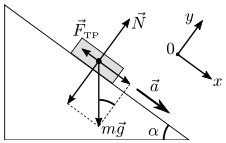
\includegraphics[scale=0.75]{pik.png}
  \captionof{figure}[LOF entry]{Векторная диаграмма сил, действующих на тело, расположенное на наклонной плоскости}   
  \label{fig:picture}
\end{center}

Поскольку в лабораторной установке коэффициент трения $\mu$ и угол $\alpha$ достаточно малы, то $\cos\alpha$ в формуле (6) можно заменить единицей. С учетом этого выражение для ускорения будет иметь вид:


\begin{equation}
a=g(\sin\alpha-\mu)
\end{equation}

Таким образом, теоретическая зависимость ускорения $a$ от $\sin\alpha$ является линейной и угловой коэффициент этой зависимости равен ускорению свободного падения $g$.




\section{Схема работы}
\begin{center}
  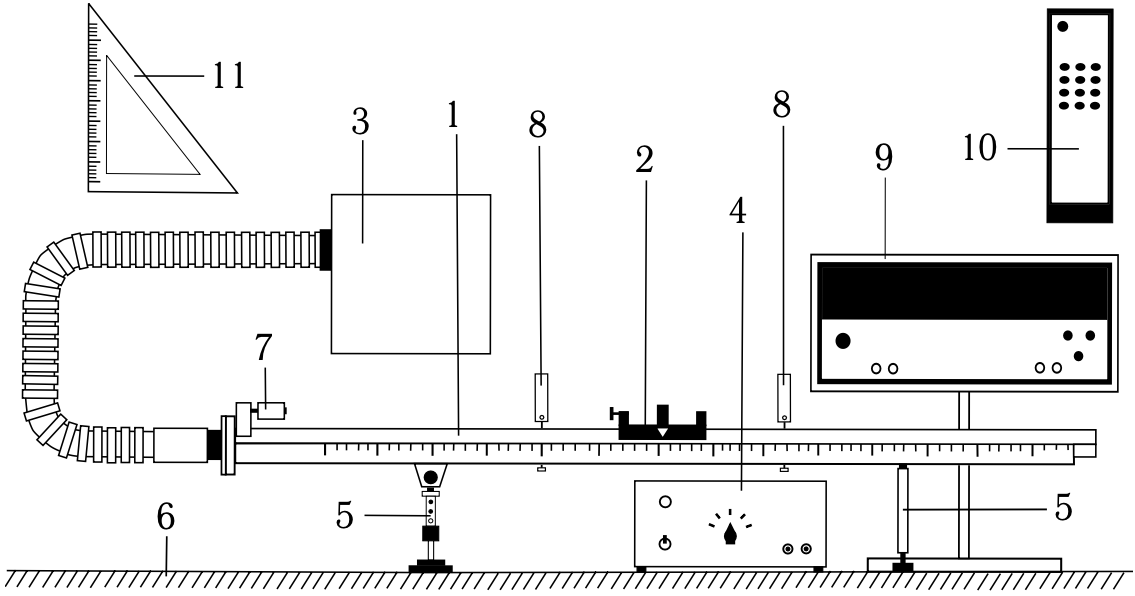
\includegraphics[scale=0.3]{pic2.png}
  \captionof{figure}[LOF entry]{Общий вид экспериментальной установки}
  \label{fig:picture}
\end{center}

\begin{enumerate}
	\item Рельс с сантиметровой шкалой на лицевой стороне
	\item Тележка
	\item Воздушный насос
	\item Источник питания насоса ВС 4-12
	\item Опоры рельса
	\item Опорная плоскость (поверхность стола)
	\item Фиксирующий электромагнит
	\item Оптические ворота
	\item Цифровой измерительный прибор ПКЦ-3
	\item Пульт дистанционного управления прибором ПКЦ-3
	\item Линейка – угольник
\end{enumerate}
По рельсу «1» скользит тележка «2». Для уменьшения трения между поверхностями рельса и тележки создается воздушная подушка с помощью воздушного насоса «3», подключенного к источнику питания «4». Электрические провода, подключающие воздушный насос к источнику питания, на рисунке не показаны. Высота рельса над опорной плоскостью «6» регулируется с помощью винтовых ножек опор «5». Электромагнит «7» фиксирует тележку в начале шкалы. Тележка снабжена флажком с черными вертикальными рисками. Цифровой измерительный прибор «9» фиксирует момент времени, скорость и ускорение тележки при прохождении флажка через оптические ворота «8». Запуск тележки и изменение режимов осуществляется пультом дистанционного управления «10». Угольник «11» используется для измерения вертикальной координаты точек рельса.

\section{Полученные данные}
\begin{center}
\begin{table}[H]
\begin{tabular}{|l|l|l|l|}
\hline

x, м & x', м & $h_0$, мм & $h_0'$, мм \\
\hline
0.22 & 1.00 & 192 & 192 \\
\hline
\end{tabular}
\end{table}
Погрешности: $\Delta x=\Delta x'=5\text{мм}, \Delta h_0=\Delta h_0'=0.5\text{мм}$.
\begin{table}[H]
\begin{tabular}{|l|l|l|l|l|}
\hline
N & x1, м & x2, м & t1, с & t2, с \\
\hline
1 & 0.15 & 0.50 & 1.2 & 2.8 \\
\hline
2 & 0.15 & 0.70 & 1.2 & 3.3 \\
\hline
3 & 0.15 & 0.90 & 1.2 & 3.9 \\
\hline
4 & 0.15 & 1.10 & 1.2 & 4.4 \\
\hline
5 & 0.15 & 1.20 & 1.3 & 4.6 \\
\hline
\end{tabular}
\end{table}
\end{center}
\begin{center}
Погрешности: $\Delta x_1=\Delta x_2=5\text{мм}, \Delta t_1=\Delta t_2=0.1\text{с}$
\end{center}
\begin{table}[ht]
\begin{tabular}{|c|c|c|c|c|}
\hline
\textbf{№ Измерения} & \textbf{$h$, мм} & \textbf{$h'$, мм}& \textbf{$t_1$, с} & \textbf{$t_2$, с} \\
\hline
1 & 202 & 192 & 1.4 & 4.5 \\
\hline
2 & 202 & 192 & 1.3 & 4.4 \\
\hline
3 & 202 & 192 & 1.3 & 4.4 \\
\hline
4 & 202 & 192 & 1.3 & 4.4 \\
\hline
5 & 202 & 192 & 1.3 & 4.4 \\
\hline
6 & 213 & 193 & 0.9 & 3.0 \\
\hline
7 & 213 & 193 & 0.9 & 3.0 \\
\hline
8 & 213 & 193 & 0.9 & 3.0 \\
\hline
9 & 213 & 193 & 0.9 & 3.0 \\
\hline
10 & 213 & 193 & 0.9 & 3.0 \\
\hline
11 & 222 & 193 & 0.7 & 2.5 \\
\hline
12 & 222 & 194 & 0.7 & 2.5 \\
\hline
13 & 222 & 194 & 0.7 & 2.5 \\
\hline
14 & 222 & 194 & 0.7 & 2.5 \\
\hline
15 & 222 & 194 & 0.7 & 2.5 \\
\hline
16 & 231 & 195 & 0.6 & 2.1 \\
\hline
17 & 231 & 195 & 0.6 & 2.1 \\
\hline
18 & 231 & 195 & 0.6 & 2.1 \\
\hline
19 & 231 & 195 & 0.6 & 2.1 \\
\hline
20 & 231 & 195 & 0.6 & 2.1 \\
\hline
21 & 242 & 195 & 0.6 & 1.9 \\
\hline
22 & 242 & 195 & 0.5 & 1.9 \\
\hline
23 & 242 & 195 & 0.5 & 1.9 \\
\hline
24 & 242 & 195 & 0.6 & 1.9 \\
\hline
25 & 242 & 195 & 0.5 & 1.9 \\
\hline
\end{tabular}
\end{table}
\begin{center}
Погрешности: $\Delta h= \Delta h'=5\text{мм}, \Delta t_1=\Delta t_2=0.1\text{с}$
\end{center}
\begin{figure}[H]
\begin{center}
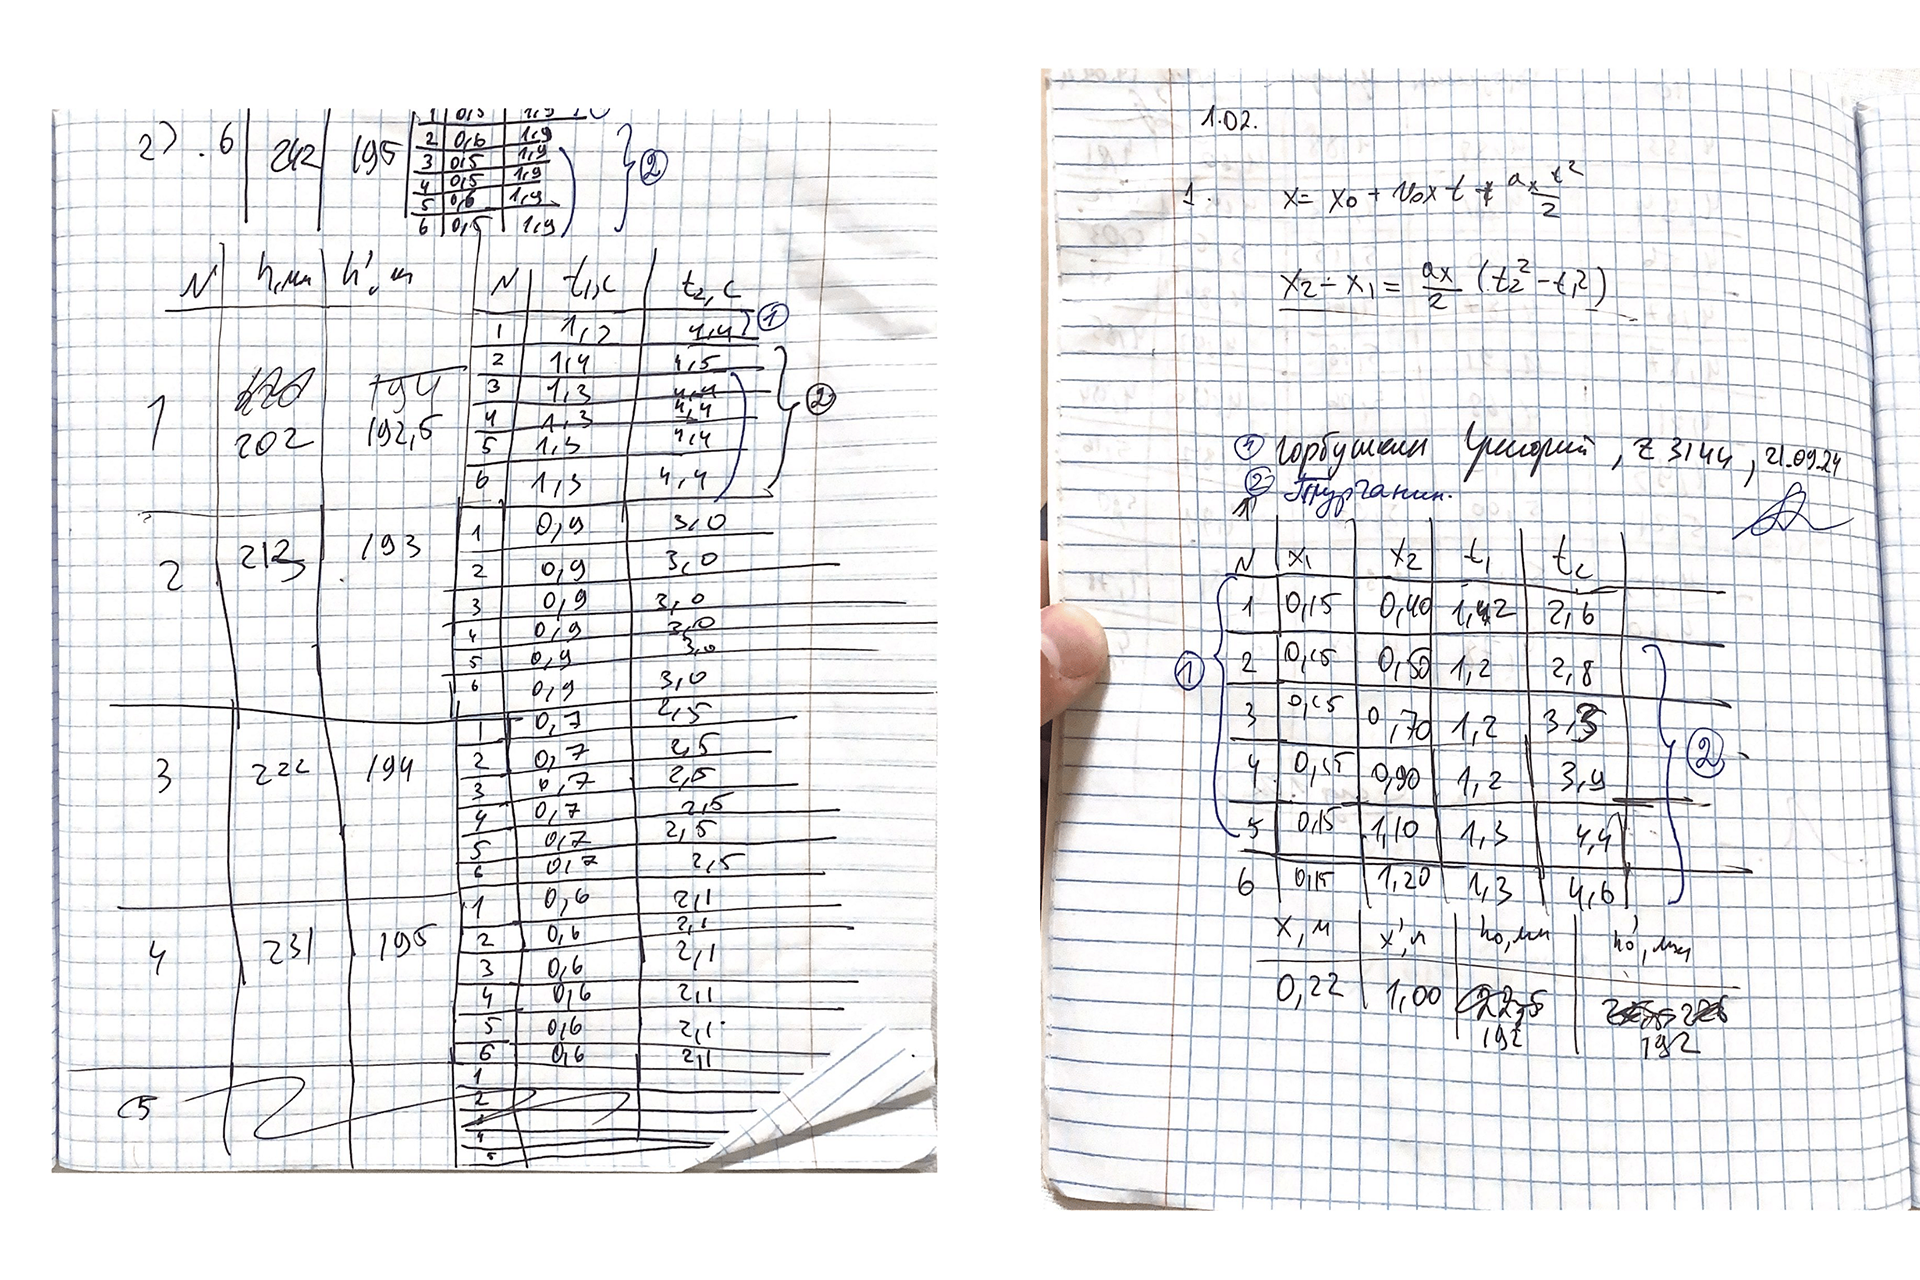
\includegraphics[scale=0.5]{1_2.png}\\
\end{center}
\end{figure}

\section{Обработка данных}
\textbf{С помощью питона обрабатываем данные и получаем}:

\begin{figure}[H]
\begin{center}
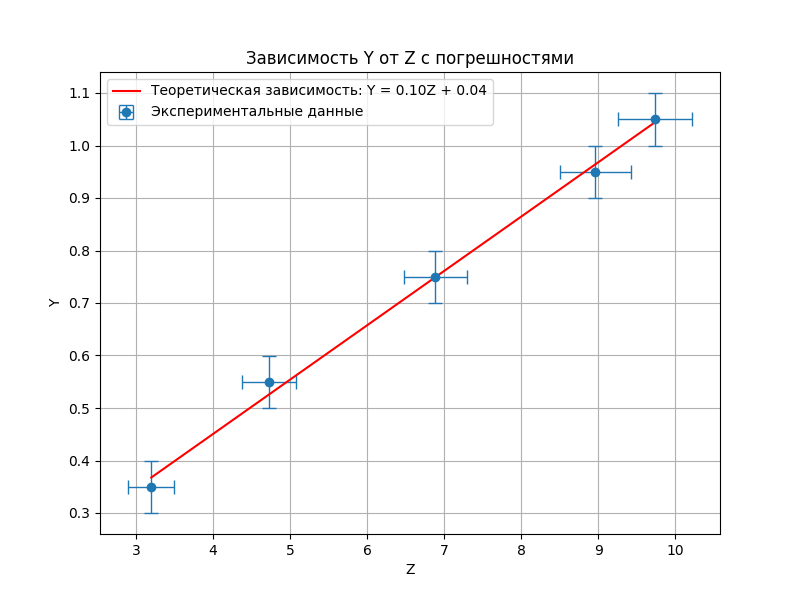
\includegraphics[scale=0.5]{Graph_1.png}
\end{center}
\end{figure}
\begin{center}

Где Y - расстояние пройденное телом, Z - разница квадратов времен, те то сколько \\
\begin{figure}[H]
\begin{center}
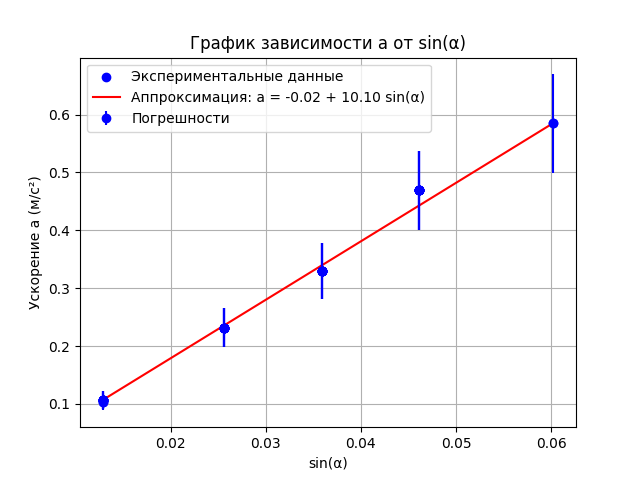
\includegraphics[scale=0.5]{plot.png}\\
\end{center}
\end{figure}

Доверительный интервал для $a$ ускорения: $[0.105, 0.111]$ \\
Относительная погрешность для $a$: 2.71 \%\\
$a = 0.108$м/с$^2$\\
Значение ускорения свободного падения: 10.10 м/с$^2$\\
Абсолютная погрешность для $g$: 0.367 м/с$^2$\\
Абсолютная погрешность от табличного значения: 0.294 м/с$^2$\\
Относительная погрешность от табличного значения: 3\% \\
\begin{align*}
\text{Доверительный интервал для } g &: 10.098 \pm 0.366 \\
\end{align*}
\end{center}

\section{Заключение}

\begin{enumerate}
	\item Из выше приведенных графиков можно сделать вывод, что движение тележки - равноускоренно, так как график - прямая.
	\item Так же можно утверждать, что ускорение свободного ускорения $g$ примерно равно 10м/с$^2$
\end{enumerate}

Причины по которым ответ может отличаться от табличного значения:
\begin{itemize}
	\item Так как все измерялось на столе который не был жестко закреплен, движение человека могли сказываться на движение тележки
	\item Сила трения на разных участках дороги может отличаться
\end{itemize}
\section{\textbf{Исправления}}
\begin{enumerate}
	\item Схема работы:
\begin{figure}[H]
\begin{center}
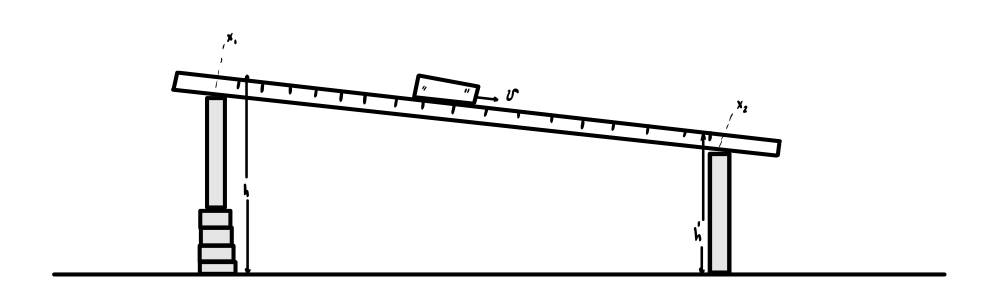
\includegraphics[scale=0.5]{pickpick.png}\\
\end{center}
\end{figure}
\item Синус угла вычисяется по формуле: $\sin{\theta}=\dfrac{h'-h}{x_2-x_1}$
\item Ускорение свободного падения складывается из ускорения от гравитации и ускорения от центростремительного ускорения:\\
	$\Delta g =GM(\dfrac{1}{R_1^2}-\dfrac{1}{R_2^2})-\dfrac{4\pi(R_1-R_2)}{T}$\\
	Тогда вклад(\%), который вносит центростремительный ускорение, равен: $\dfrac{\dfrac{4\pi(R_1-R_2)}{T}}{GM(\dfrac{1}{R_1^2}-\dfrac{1}{R_2^2})-\dfrac{4\pi(R_1-R_2)}{T}}\cdot100$

\end{enumerate}
\end{document}





